\documentclass[twocolumn,DIV18]{scrartcl}
\usepackage{refcheck}
\usepackage{amsmath}
\usepackage{graphicx}
\newcommand{\abs}[1]{\lvert #1 \rvert}
\renewcommand{\(}{\left(}
\renewcommand{\)}{\right)}
%\newcommand{\eqref}[1]{(\ref{#1})}
\begin{document}
\title{Equidistant spiral sampling}
\author{Martin Kielhorn}
\maketitle
\section{Introduction}
We want to illuminate different points in the back focal plane of a
micro objective. Its convenient to have a 1D indexing scheme for these
points. Due to the circular symmetry a spiral sampling [1983Ahn] comes
to mind. 

\section{Archimedes Spiral}
An Archimedes spiral in polar coordinates $(r,\theta)$ is defined like
this:
\begin{align} \label{eqn:def}
  r(\theta)=a\,\theta.
\end{align}
The step height $h$ of the spiral is given by
\begin{align}
  h=\abs{r(\theta)-r(\theta+2\pi)}=r(2\pi)=2\pi a.
\end{align}
\section{Equidistance sampling}
We want to start sampling in the center at $r(0)=0$ and sample the arc
length of the spiral with equidistant points. The arc length of an
archimedes spiral is [Weisstein]:
\begin{align} \label{eqn:arclength}
  s(\theta)=\frac{a}{2}\(p\,\theta + \log(p\,\theta)\)\quad\textrm{with}\quad
  p=\sqrt{1+\theta^2}.
\end{align}
The arc length $\Delta s$ between successive points along the spiral
should be equal to the step height $h$. Starting from the central
point $\theta_0=0$ the arc length where to sample the $i-$th point can
be obtained by inverting equation \eqref{eqn:arclength}:
\begin{align}
  \theta_i=\theta(i\,\Delta s).
\end{align}
This inversion can be done efficiently with Newton interation
[Wikipedia]:
\begin{align}
  x_0&=1,\\
  x_{n+1}&=x_n-\frac{f(x)}{f'(x)}.
\end{align}
Here we introduce the function $f(\theta)$ that vanishes at a given arc
length $s$ and its derivative $f'(\theta)$:
\begin{align}
  \label{eqn:f}
  f(\theta)&=\frac{a}{2}\(p\,\theta+\log(p\,\theta)\)-s,\\
  f'(\theta)&=\frac{\partial f(\theta)}{\partial \theta}=
  \frac{a}{2}\frac{(1+2\theta^2)(1+p\theta)}{p^2 \theta}.
\end{align}
\section{Filling the back focal plane}
We want to find the coordinates of equaly distributed sampling points
along the arc length inside of a circle with radius R. We put the
first sampling point $\theta_0=0$ in the center and the last point
$\theta_n$ on the periphery of the circle. By definition
\eqref{eqn:def} of the spiral we know
\begin{align}
  \theta_n=R/a.
\end{align}
Now we obtain the arc length $s(\theta_n)$ of the spiral contained
inside the circle via \eqref{eqn:arclength}. Dividing by the number of
sub-intervals gives the apropriate sampling step $\Delta s =
s(\theta_n)/(n-1)$.

Note that we are only interested in solutions with $\Delta s=h$. We
want the sampling step to be equal to the step height $h=2\pi a$ of
the spiral. We therefor need to find the zero of the function:
\begin{align}
  g(a)&=\frac{s(\theta_n)}{n-1}-2\pi a\\
  &=\frac{a}{2}\frac{p\theta_n+\log p\theta_n}{n-1}-2\pi a\\
  &=\frac{a}{2}\frac{\sqrt{1+\frac{R^2}{a^2}}\frac{R}{a}+
    \log\(\sqrt{1+\frac{R^2}{a^2}}\frac{R}{a}\)}{n-1}-2\pi a.
\end{align}
Actually we know $a\not =0$ so we can transform the function to
simplify its derivative:
\begin{align}
  g_1(a)&=\underbrace{\sqrt{1+\frac{R^2}{a^2}}}_{p_1}\frac{R}{a}+
  \log\(\sqrt{1+\frac{R^2}{a^2}}\frac{R}{a}\)-4\pi (n-1),\\
  g_1'(a)&=-\frac{R^3}{p_1}\frac{1}{a^4}-\frac{R^2}{p_1^2}\frac{1}{a^3}-R
    p_1\frac{1}{a^2}-\frac{1}{a}.
\end{align}
\begin{figure}[h]
  \begin{center}
    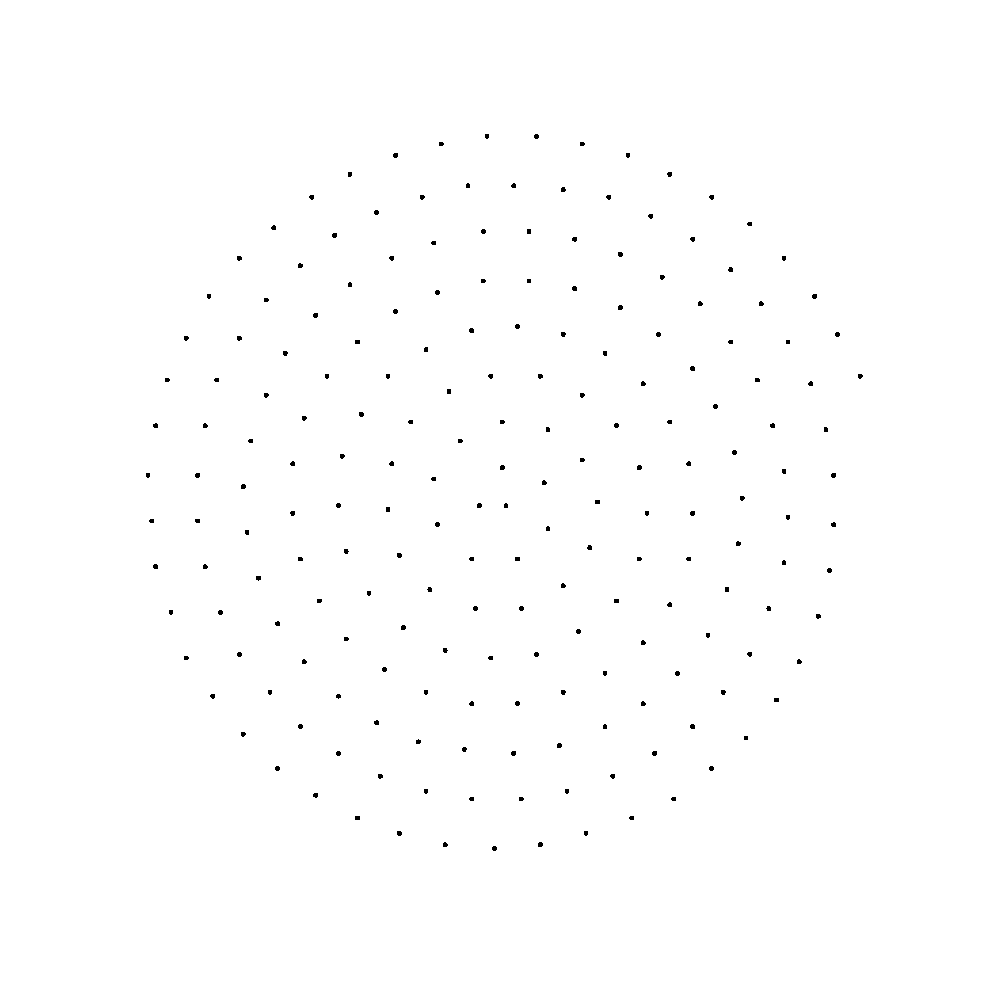
\includegraphics[width=.3\columnwidth]{200}
    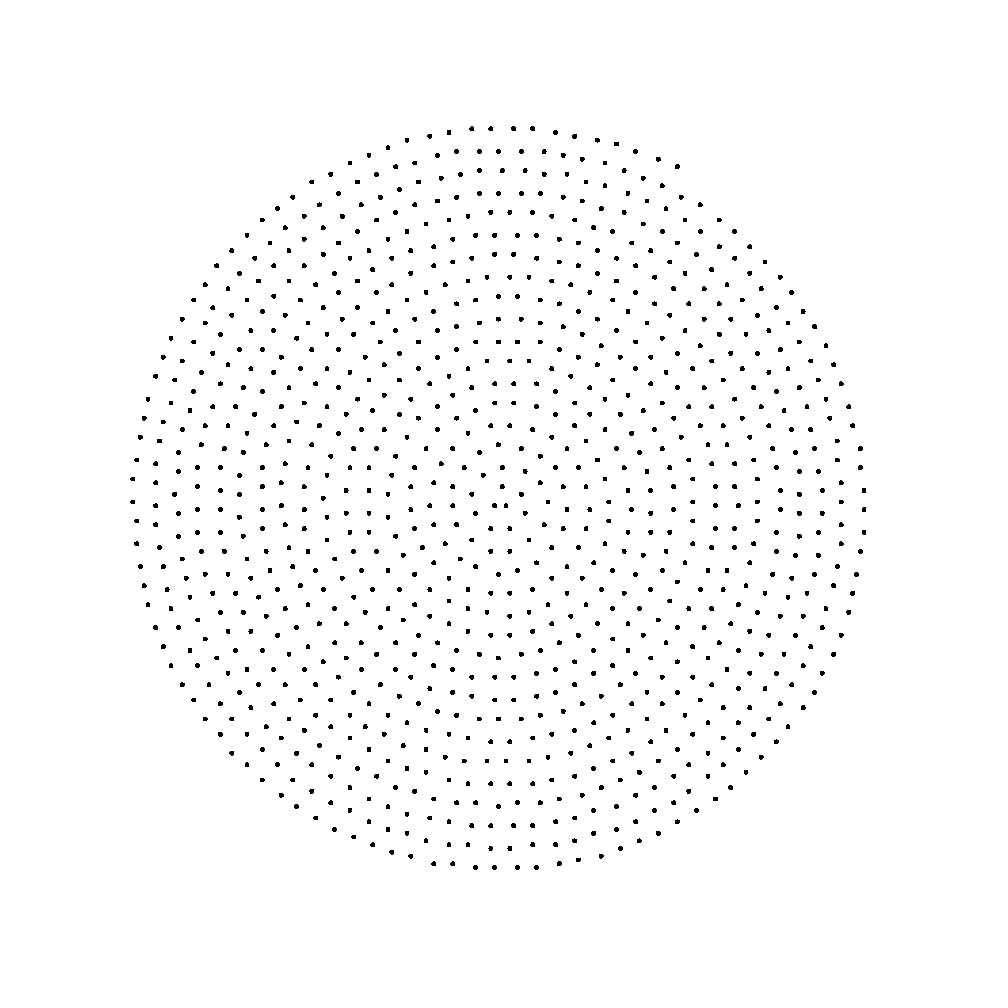
\includegraphics[width=.3\columnwidth]{1000}
    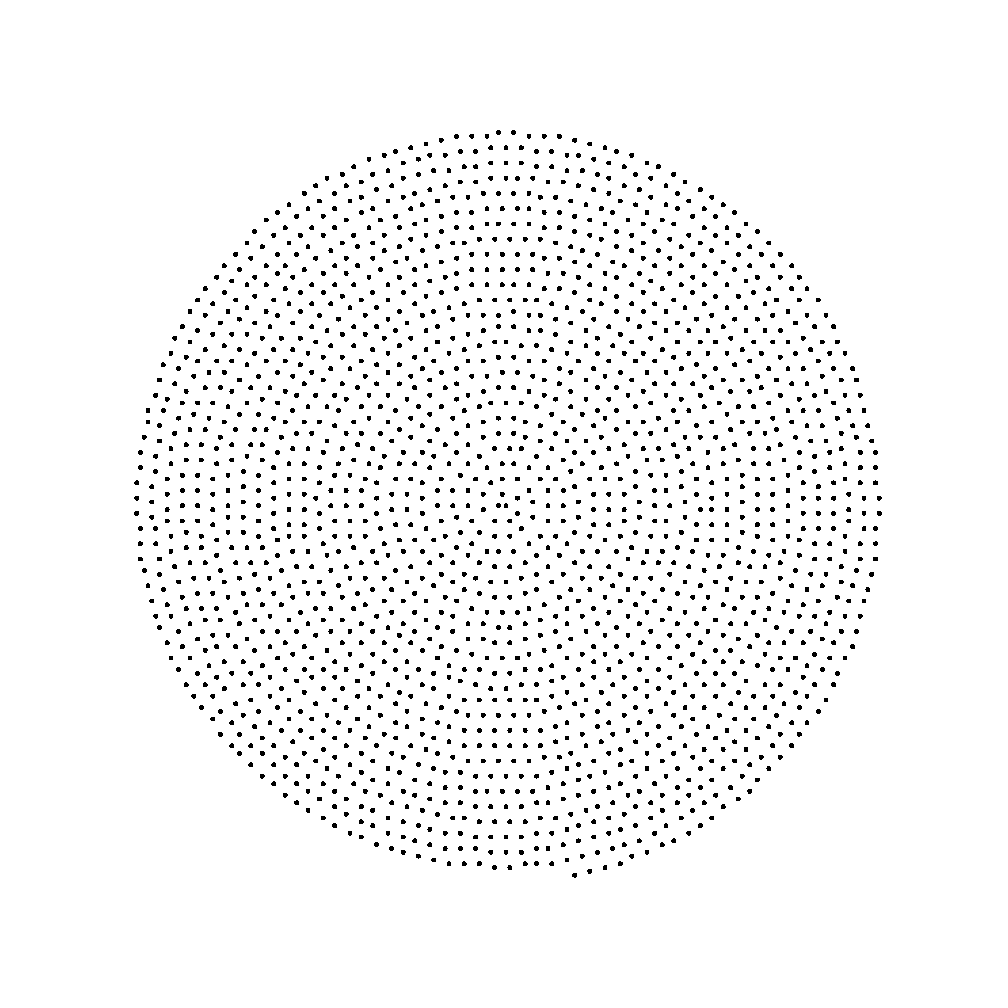
\includegraphics[width=.3\columnwidth]{2000}
  \end{center}
  \caption{Equidistant sampling of a circle of the same diameter
    $R=100$ with 200 (left), 1000 (middle) and 2000 (right)
    points.}
\end{figure}
\end{document}
%% FindRoot[{a x == R, a/2 (Sqrt[1+x^2]x+Log[Sqrt[1+x^2]x]) == n * 2 pi a + R/a}, {{x, 1}, {a, 1}}]

%% @ARTICLE{4307732,
%% author={Ahn, C. B. and Kim, J. H. and Cho, Z. H.},
%% journal={Medical Imaging, IEEE Transactions on}, title={High-Speed Spiral-Scan Echo Planar NMR Imaging-I},
%% year={1986},
%% month={mar.},
%% volume={5},
%% number={1},
%% pages={2 -7},
%% keywords={},
%% doi={10.1109/TMI.1986.4307732},
%% ISSN={0278-0062},}

%% Weisstein, Eric W. "Archimedes' Spiral." From MathWorld--A Wolfram
%% Web Resource. http://mathworld.wolfram.com/ArchimedesSpiral.html


%% http://en.wikipedia.org/wiki/Newton's_method

%% multidimensional newton method
%% http://math.fullerton.edu/mathews/n2003/NewtonSystemMod.html
